\graphicspath{ {../../images/} }
\usetikzlibrary{external}
\usepackage{changepage}

\newlength{\offset}

\title{ITC8280 Fundamentals of Cryptography}
\subtitle{Certificate validity, eIDAS \& qualified signatures}
\date{\today}
\author{Taaniel Kraavi}
\institute%
{%
  \textit{School of Information Technologies}\\
  \textit{Tallinn University of Technology}
}

\begin{document}
\begin{frame}
  \titlepage
\end{frame}

\begin{frame}{Refresher on PKI}
  Hierarchical trust model:
  \begin{itemize}[<+(1)->]
    \item Root CA self-signs their own root certificate(s) (trust-anchor)
    \item Root certificates used to certify subordinate/intermediate certificates
    \item Subordinates issue end-entity certificates or certify other subordinates
  \end{itemize}

  \vspace*{1em}

  \pause
  A root certificate is linked to end-entity certificates through intermediate certificates.
  \begin{itemize}[<+(1)->]
    \item This forms the certificate chain
  \end{itemize}
\end{frame}

\begin{frame}{Refresher on PKI}
  Two main authorities:
  \begin{itemize}[<+(1)->]
    \item Certification Authority (CA): issues \& manages certificates
    \item Registration Authority (RA): verifies applicant identities
  \end{itemize}
\end{frame}

\begin{frame}{Getting certificates}
  Applying for a digital certificate:
  \begin{enumerate}[<+(1)->]
    \item Prepare a Certificate Signing Request (CSR)
    \item Send the CSR to the CA
    \item The CA returns the certificate
  \end{enumerate}

  \vspace*{1em}

  \pause
  Main questions:
  \begin{itemize}
    \item CSR contents?
    \item Proof of origin?
    \item Automation?
  \end{itemize}
\end{frame}

\begin{frame}{PKCS\#10 CSR}
  The most common CSR format is PKCS\#10 (\href{https://datatracker.ietf.org/doc/html/rfc2986}{RFC 2986}):
  \begin{itemize}[<+(1)->]
    \item Certification request info
    \begin{itemize}
      \item Subject information
      \item Subject public key
      \item Additional attributes (optional)
    \end{itemize}
    \item Signature algorithm identifier
    \item Signature (of the subject) on the certification request info
  \end{itemize}

  \vspace*{1em}

  \pause
  PKCS\#10 does not specify how the CA verifies the requester.
\end{frame}

\begin{frame}{Certificate management protocols (pt. 1)}
  Certificate Management Protocol (CMP)
  \begin{itemize}[<+(1)->]
    \item Full certificate lifecycle: enrolment, renewal, revocation
    \item Transport agnostic; flexible but complex
    \item Use when full lifecycle control is needed (e.g.\ enterprise PKI)
  \end{itemize}

  \vspace{1em}

  \pause
  Enrolment over Secure Transport (EST) {\scriptsize successor to SCEP (considered legacy, except by Microsoft\dots)}
  \begin{itemize}[<+(1)->]
    \item Certificate enrolment and renewal, but not revocation
    \item TLS transport; mTLS or enrolment code authentication
    \item Use when provisioning is enough; popular for MDM, IoT
  \end{itemize}
\end{frame}

\begin{frame}{Certificate management protocols (pt. 2)}
  Automated Certificate Management Environment (ACME)
  \begin{itemize}[<+(1)->]
    \item Automated certificate issuance and renewal for web servers
    \item Challenge-response authentication
    \item Use for TLS certificates
  \end{itemize}

  \pause
  We will talk more about ACME next week.
\end{frame}

\begin{frame}{Certification path validation}
  \href{https://datatracker.ietf.org/doc/html/rfc5280}{RFC 5280} describes PKIX certification path validation
  \begin{itemize}[<+(1)->]
    \item Given a trust anchor and a certification path $C_1, \dots, C_n$, verify that
    \begin{enumerate}[<+(1)->]
      \item $C_{i+1}$ is issued\textsuperscript{*} by $C_i$ for $i\in\{1, \dots, n-1\}$ \hfil {\scriptsize \textsuperscript{*}(name match and valid signature)}
      \item $C_1$ is issued\textsuperscript{*} by the trust anchor
      \item $C_n$ is the validation target
      \item $C_i$ was valid at the verification time for $i\in\{1, \dots, n\}$
    \end{enumerate}
    \item Extensions must be enforced
    \item Policies and status may be checked (policy-dependent)
    \item Other standards may further tighten validation requirements
  \end{itemize}
\end{frame}

\begin{frame}{Certificate status}
  What if\dots
  \begin{itemize}[<+(1)->]
    \item The end-entity is compromised?
    \item The certificate was mis-issued?
    \item The CA is compromised?
  \end{itemize}

  \vspace*{1em}

  \pause
  We need a mechanism for revoking certificates before their natural expiry.
\end{frame}

\begin{frame}{Certificate Revocation Lists (CRL)}
  List of certificates revoked by a CA:
  \begin{itemize}[<+(1)->]
    \item Revocation states: revoked (permanent) \& certificate hold (temporary)
    \begin{itemize}
      \item Revocation reason is optional
      \item Revoked certificates are typically removed after expiry
    \end{itemize}
    \item Periodically issued by the CA
    \begin{itemize}
      \item May be issued by a delegated CRL issuer
      \item \texttt{thisUpdate} field: when the CRL was published
      \item \texttt{nextUpdate} field: CRL is considered stale after this time
    \end{itemize}
    \item Certificate field: CRL Distribution Points
  \end{itemize}

  \pause
  The \emph{relying party} must download and process the entire CRL.
\end{frame}

\begin{frame}{Liability and CRLs}
  \pause
  Who is liable during the \enquote{revocation lag}?
  \begin{itemize}[<+(1)->]
    \item Certificate revoked but not yet published in the CRL
    \item Should the RP wait until the next CRL update?
    \item No clear legal or technical answer
  \end{itemize}

  \pause
  Critical use cases require timely certificate status information.
\end{frame}

\begin{frame}{Online Certificate Status Protocol (OCSP)}
  OCSP allows us to obtain the revocation status of a specific certificate (\href{https://datatracker.ietf.org/doc/html/rfc6960}{RFC 6960}).

  \vspace*{0.5em}

  \pause
  Certificate status endpoints are called OCSP \emph{responders}.
  \begin{itemize}[<+(1)->]
    \item Endpoint(s) specified in the certificate (Authority Information Access extension)
    \item Either CA or CA-authorised (delegated) responders
    \item Delegated responder certificate must have the OCSP Signing EKU
  \end{itemize}

  \vspace*{0.5em}

  \pause
  Response status: \enquote{good}, \enquote{revoked}, \enquote{unknown}
  \begin{itemize}[<+(1)->]
    \item Unknown: the responder does not recognise the certificate
  \end{itemize}
\end{frame}

\begin{frame}{OCSP vs.\ CRL}
  Client benefits:
  \begin{itemize}[<+(1)->]
    \item Per-certificate queries -- no need to download the entire CRL
    \item More timely status information
    \begin{itemize}
      \item Responses may be cached, and therefore not fresh
      \item The OCSP nonce extension (if supported) helps with freshness
    \end{itemize}
    \item Smaller responses -- easier to parse
  \end{itemize}

  \vspace*{0.5em}

  \pause
  CA burden:
  \begin{itemize}[<+(1)->]
    \item Must operate a live responder
    \item Higher load compared to periodic CRL publishing
  \end{itemize}
\end{frame}

\begin{frame}{OCSP pitfalls}  
  \pause
  Replay attacks:
  \begin{itemize}[<+(1)->]
    \item For efficiency, OCSP responses are often pre-signed
    \item Check the OCSP issuing time (thisUpdate \& nextUpdate fields)
    \item OCSP nonce extension helps: random nonce for the request
  \end{itemize}

  \vspace*{0.5em}

  \pause
  Privacy concerns:
  \begin{itemize}[<+(1)->]
    \item Requires contacting the CA's responder, possibly over plaintext
    \item Leaks query information (e.g. websites browsed)
  \end{itemize}
\end{frame}

\begin{frame}{OCSP stapling}
  \pause
  Include an OCSP response with the data responses:
  \begin{itemize}[<+(1)->]
    \item Server periodically makes OCSP requests to the CA itself
    \item Server sends the requests back with the requested data
    \item OCSP response still signed by the responder
    \item E.g. website serving the OCSP response alongside the HTTPS certificates
  \end{itemize}

  \pause
  Formally known as the \enquote{TLS Certificate Status Request} extension.
\end{frame}

\begin{frame}{OCSP stapling}
  \begin{figure}
    \centering
    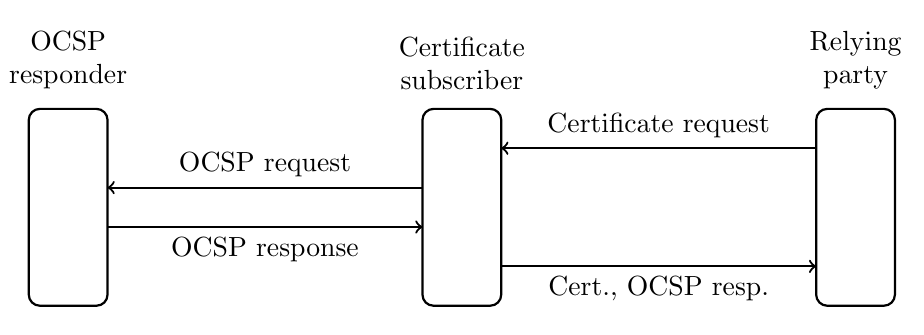
\begin{tikzpicture}
      \draw[rounded corners,thick] (0, 0) rectangle  ++(1,-2.5);
      \draw[rounded corners,thick] (5, 0) rectangle ++(1,-2.5);
      \draw[rounded corners,thick] (10, 0) rectangle ++(1,-2.5);

      \node[label={[align=center]Certificate\\subscriber}] at (5.5, 0) {};

      % Set the picture size to everything drawn so far.
      % This ignores the label sizes for centering.
      \useasboundingbox (current bounding box);
    
      \node[label={[align=center]OCSP\\responder}] at (0.5, 0) {};
      \node[label={[align=center]Relying\\party}] at (10.5, 0) {};
    
      \draw[<-,thick] (6, -0.5) -- (10, -0.5) node[midway,above] {Certificate request};
      \draw[<-,thick] (1, -1) -- (5, -1) node[midway,above] {OCSP request};
      \draw[->,thick] (1, -1.5) -- (5, -1.5) node[midway,below] {OCSP response};
      \draw[->,thick] (6, -2) -- (10, -2) node[midway,below] {Cert., OCSP resp.};
    \end{tikzpicture}
  \end{figure}
\end{frame}

\begin{frame}{Missing staple}
  \pause
  What to do if the cert is not stapled?
  \begin{itemize}[<+(1)->]
    \item Query the responder directly
    \item What if an attacker drops the requests?
  \end{itemize}

  \vspace*{0.5em}
  
  \pause
  OCSP \enquote{must staple} extension
  \begin{itemize}[<+(1)->]
    \item Fail the task if no OCSP response provided
    \item Prevents some downgrade attacks
  \end{itemize}

  \vspace*{0.5em}

  \pause
  CAs do not typically like OCSP, and stapling is not very popular
\end{frame}

\begin{frame}{Disclaimer}
  Everything that follows is grossly oversimplified.
  \pause
  \begin{itemize}
    \item Legal rather than cryptographic topics
    \item Numerical identity vs. legal identity
    \item Laws attach legal validity to technical validity
  \end{itemize}
\end{frame}

\begin{frame}{eIDAS}
  Electronic Identification, Authentication and Trust Services
  \begin{itemize}[<+(1)->]
    \item EU regulation: directly applicable to all member states
    \item Interoperability of electronic identification (eID) \& trust services
    \item Legal validity
    \item National identity providers (IdP)
  \end{itemize}

  \vfill

  \pause
  eIDAS \enquote{2.0} amends the original regulation.
  \begin{itemize}[<+(1)->]
    \item \href{https://eur-lex.europa.eu/eli/reg/2024/1183/oj}{Regulation (EU) 2024/1183}
    \item Introduces digital identity wallets
    \item The amendments are out of our scope
  \end{itemize}
\end{frame}

\begin{frame}{eIDAS eID}
  eIDAS eID online service access:
  \begin{enumerate}[<+(1)->]
    \item A citizen requests an on-line service in another Member State.
    \item The citizen is requested to authenticate themselves by the on-line service.
    \item The citizen chooses to authenticate with an eIDAS eID.
    \item The authentication request is sent to the citizen's country for authentication.
    \item The authentication result is returned to the service provider.
    \item Authentication is complete and the citizen can proceed.
  \end{enumerate}

  \pause
  {\scriptsize Source: \href{https://ec.europa.eu/digital-building-blocks/sites/display/DIGITAL/eID}{\textit{Digital Europe Programme eID FAQ}}}

  \pause
  See also: \href{https://www.eid.as/tsp-map/}{eIDAS eID map}
\end{frame}

\begin{frame}{Trust services}
  Trust services are electronic services that help various parties make \emph{binding} decisions.
  E.g.
  \begin{itemize}[<+(1)->]
    \item Timestamping
    \item E-signing
    \item Digital authentication
    \item Validity confirmation
    \item \dots
  \end{itemize}
\end{frame}

\begin{frame}{EU/EEA Trusted List}
  EU/EEA Trusted List Browser:
  \begin{itemize}[<+(1)->]
    \item Qualified status granted by supervisory body
    \item Member states maintain their own trusted lists
    \item EU maintains the list of trusted lists (EU-level PKI)
    \item {\scriptsize \url{https://eidas.ec.europa.eu/efda/tl-browser/}}
    \item {\scriptsize \url{https://ec.europa.eu/tools/lotl/eu-lotl.xml}}
  \end{itemize}
\end{frame}

\begin{frame}{eIDAS signature levels}
  Article 3:
  \settowidth{\offset}{10}
  \addtolength{\leftmargini}{\offset}
  \begin{itemize}[<+(1)->]
    \item[(10)] \enquote{electronic signature (ES)}
    \item[(11)] \enquote{advanced electronic signature (AdES)}
    \item[(12)] \enquote{qualified electronic signature (QES)}
  \end{itemize}
\end{frame}

\begin{frame}{Electronic signature (ES)}
  \enquote{electronic signature (ES)} means data in electronic form which is attached to or logically associated with other data in electronic form and which is used by the signatory to sign;
\end{frame}

\begin{frame}{Advanced electronic signature (AdES)}
  \enquote{advanced electronic signature (AdES)} means an electronic signature which meets the requirements set out in Article 26;
  \settowidth{\offset}{26.1}
  \addtolength{\leftmargini}{\offset}
  \begin{enumerate}[<+(1)->]
    \item[(26.a)] it is uniquely linked to the signatory;
    \item[(26.b)] it is capable of identifying the signatory;
    \item[(26.c)] it is created [\dots] under his sole control; and
    \item[(26.d)] [\dots] any subsequent change in the data is detectable.
  \end{enumerate}
\end{frame}

\begin{frame}{Qualified electronic signature (QES)}
  \enquote{qualified electronic signature (QES)} means an \emph{advanced electronic signature} that is created by a \emph{qualified electronic signature creation device}, and which is based on a \emph{qualified certificate} for electronic signatures;
  \begin{itemize}[<+(1)->]
    \item qualified certificate: certificate issued by a qualified trust service provider
  \end{itemize}

  \vfill

  \pause
  AdES/QC: advanced electronic signature (AdES) based on a qualified certificate.
\end{frame}

\begin{frame}{Signature levels simplified (pt. 1)}
  \pause
  Electronic signatures (ES):
  \begin{itemize}[<+(1)->]
    \item Data used by a signatory to express signing \emph{intent}
    \item E.g. signing an email with your name
  \end{itemize}

  \vspace*{1em}

  \pause
  Advanced electronic signature (AdES):
  \begin{itemize}[<+(1)->]
    \item Electronic signature \emph{uniquely} linked to an \emph{identifiable} entity
    \item Must assert the \emph{integrity} of signed data
    \item E.g. signature issued with OpenSSL for a published certificate
    \item If the certificate is qualified: AdES/QC
  \end{itemize}
\end{frame}

\begin{frame}{Signature levels simplified (pt. 2)}
  \pause
  Qualified electronic signature
  \begin{itemize}[<+(1)->]
    \item AdES where the certificate and signing device are qualified
    \item E.g. digital signatures issued with an Estonian ID card
  \end{itemize}

  \vspace*{1em}

  \pause
  In Estonian \enquote{digiallkiri} is supposed to refer to a QES.

  The term for a cryptographic digital signature is \enquote{(digi)signatuur}.
\end{frame}

\begin{frame}{Qualified Signature Creation Devices (QSCD)}
  \pause
  eIDAS Annex II:
  \settowidth{\offset}{1.a}
  \addtolength{\leftmargini}{\offset}
  \begin{enumerate}[<+(1)->]
    \item[(1.a)] the confidentiality of the electronic signature creation data [\dots] is reasonably assured;
    \item[(1.b)] the [\dots] data [\dots] can practically occur only once;
    \item[(1.c)] the [\dots] data [\dots] cannot [\dots] be derived and the electronic signature is reliably protected against forgery [\dots];
    \item[(1.d)] the [\dots] data [\dots] can be reliably protected by the legitimate signatory against use by others.
  \end{enumerate}

  \pause
  TL;DR: It should only be possible to issue signatures when possessing the device, and its use should be restricted (e.g. protected by a PIN).
\end{frame}

\begin{frame}{Validating Qualified Electronic Sigantures}
  \href{https://eur-lex.europa.eu/legal-content/EN/TXT/HTML/?uri=CELEX\%3A32014R0910\#d1e2594-73-1}{Article 32} specifies how to validate QES signatures.
  \begin{itemize}[<+(1)->]
    \item Quite tricky!
  \end{itemize}

  \vspace*{1em}

  \pause
  \href{https://eur-lex.europa.eu/legal-content/EN/TXT/HTML/?uri=CELEX:32014R0910\#d1e2664-73-1}{Article 33} describes a Qualified Validation Service:
  \begin{itemize}
    \item Automated validation process
    \item Search for providers \href{https://eidas.ec.europa.eu/efda/trust-services/browse/eidas/tls/search/type?step=1}{\textit{here}}
    \item Not always available, in which case use a library
  \end{itemize}

  \vspace*{1em}

  \pause
  (\href{https://eur-lex.europa.eu/legal-content/EN/TXT/HTML/?uri=OJ:L\_202401183\#d1e3370-1-1}{\textit{eIDAS 2.0 amendments}})
\end{frame}

\begin{frame}{Legal effects of electronic signatures}
  \pause
  Article 25:
  \begin{enumerate}
    \setcounter{enumi}{1}
    \item A qualified electronic signature shall have the equivalent legal effect of a handwritten signature.
  \end{enumerate}

  \vspace*{1em}

  \pause
  Legal implication:
  \begin{itemize}[<+(1)->]
    \item Accusing party needs not prove that an entity issued the signature.
    \item Issuer has to prove that they did not issue the signature.
    \item $\implies$ legal non-repudiation
    \item Article 13, paragraph 1
  \end{itemize}
\end{frame}

\begin{frame}{Digital vs. electronic signature}
  Digital signature:
  \begin{itemize}[<+(1)->]
    \item Cryptographic concept
    \item A tool to prove integrity and provenance
  \end{itemize}

  \vspace*{1em}

  \pause
  Electronic signature:
  \begin{itemize}[<+(1)->]
    \item Legal concept defined in eIDAS
    \item Signature on some data: intent of signatory to associate with this data
    \item Not necessarily cryptographic (e.g. name on an email)
  \end{itemize}

  \vspace*{1em}

  \pause
  Not all electronic signatures are digital signatures!
\end{frame}

\begin{frame}{Trusted timestamping}
  \pause
  Article 3:
  \settowidth{\offset}{33}
  \addtolength{\leftmargini}{\offset}
  \begin{enumerate}
    \item[(33)] \enquote{electronic time stamp} means data in electronic form which binds other data in electronic form to a particular time establishing evidence that the latter data existed at that time;
  \end{enumerate}

  \pause
  Article 41:
  \begin{itemize}
    \setcounter{enumi}{1}
    \item A qualified electronic time stamp shall enjoy the presumption of the accuracy of the date and the time it indicates and the integrity of the data to which the date and time are bound.
  \end{itemize}
\end{frame}

\begin{frame}{Trusted timestamping}
  \pause
  Signed statement by a Time Stamping Authority (TSA):
  \begin{itemize}[<+(1)->]
    \item TSAs must use an accurate time source
    \item TSAs must log issued timestamps
  \end{itemize}

  \vspace*{0.5em}

  \pause
  \href{https://datatracker.ietf.org/doc/html/rfc3161}{RFC 3161}: Internet X.509 Public Key Infrastructure Time-Stamp Protocol

  \vspace*{0.5em}

  \pause
  Time does not exist in cryptography:
  \begin{itemize}[<+(1)->]
    \item Relative temporal ordering is the best we can achieve
    \begin{itemize}
      \item E.g. which document was signed earlier (earlier in a chain)
    \end{itemize}
    \item Even chain-based TSAs require \enquote{trust} (e.g. Guardtime)
  \end{itemize}
\end{frame}

\begin{frame}{ETSI signature conformance levels}
  Incremental requirements for long-term signature validity:
  \begin{enumerate}[<+(1)->]
    \item B-B: valid until the signature certificate is valid
    \begin{itemize}
      \item \enquote{Short-term} signatures
    \end{itemize}
    \item B-T: prove that the signature existed at a certain time
    \begin{itemize}
      \item Trusted token: TSA-signed time-stamp and signature digest
    \end{itemize}
    \item B-LT: long-term availability of validation material
    \begin{itemize}
      \item Include also the OCSP/CLR status + chain at the time
    \end{itemize}
    \item B-LTA: long-term availability and integrity of validation material
    \begin{itemize}
      \item Include a \enquote{document-time-stamp} token
      \item Encompasses also the validation material
      \item Tokens can be subsequently added to prolong validity
    \end{itemize}
  \end{enumerate}
\end{frame}

\begin{frame}{ETSI signature standards (eIDAS versions)}
  ETSI specifies three formats for AdES+\dots
  \begin{itemize}[<+(1)->]
    \item XML advanced electronic signature (XAdES)
    \begin{itemize}
      \item \href{http://www.etsi.org/deliver/etsi_ts/103100_103199/103171/02.01.01_60/ts_103171v020101p.pdf}{ETSI TS 103 171 v.2.1.1}
    \end{itemize}
    \item CMS advanced electronic signature (CAdES)
    \begin{itemize}
      \item \href{http://www.etsi.org/deliver/etsi_ts/103100_103199/103173/02.02.01_60/ts_103173v020201p.pdf}{ETSI TS 103 173 v.2.2.1}
    \end{itemize}
    \item PDF advanced electronic signature (PAdES)
    \begin{itemize}
      \item \href{http://www.etsi.org/deliver/etsi_ts/103100_103199/103172/02.02.02_60/ts_103172v020202p.pdf}{ETSI TS 103 172 v.2.2.2}
    \end{itemize}
  \end{itemize}

  \pause
  \dots and one container format
  \pause
  \begin{itemize}
    \item Associated Signature Container (ASiC)
    \item \href{http://www.etsi.org/deliver/etsi_ts/103100_103199/103174/02.02.01_60/ts_103174v020201p.pdf}{ETSI TS 103 174 v.2.2.1}
  \end{itemize}
\end{frame}

\begin{frame}{XAdES}
  XML advanced electronic signature
  \begin{itemize}[<+(1)->]
    \item Based on XML digital signatures (XMLDSig)
    \item W3C recommendation: XML Signature Syntax and Processing
    \item Human and machine readable
    \item Signs any document/data (including binary data)
    \item Can sign multiple files with one signature
  \end{itemize}    
\end{frame}

\begin{frame}{CAdES}
  CMS advanced electronic signature
    \begin{itemize}[<+(1)->]
      \item Cryptographic Message Syntax (CMS)
      \item Signs only binary data, signatures not human readable
      \item Lacks XAdES features (e.g. multi-document signing), and offers none more
    \end{itemize}
\end{frame}

\begin{frame}{PAdES}
  PDF advanced electronic signature
  \begin{itemize}[<+(1)->]
    \item Signatures embedded within the PDF
    \item Included in the ISO PDF standard
    \item Signing and verification included in PDF software\textsuperscript{*}
  \end{itemize}

  \vspace*{1em}

  \pause
  PAdES is much more limited than X/CAdES, but is more \enquote{portable}.
\end{frame}

\begin{frame}{XAdES signing modes}
  Two signing modes:
  \begin{itemize}[<+(1)->]
    \item Detached: data is separate from the signature
    \begin{itemize}
      \item The original data is not modified
    \end{itemize}
    \item Encapsulated: XML file encapsulating the data
    \begin{itemize}
      \item Not usable/practical with all types of data
      \item Signature and data in the same file
    \end{itemize}
  \end{itemize}

  \vspace*{1em}

  \pause
  How to prevent signature/data loss for detached signatures?
\end{frame}

\begin{frame}{Associated Signature Containers (ASiC)}
  Data container grouping data objects with signatures and/or timestamps.
  \begin{itemize}[<+(1)->]
    \item Associates detached signatures with referenced data
    \begin{itemize}
      \item Aims to prevent the loss of signatures/data
      \item Can group signatures of multiple signatories
    \end{itemize}
    \item ZIP format
    \item Developed by ETSI
    \begin{itemize}
      \item \href{http://www.etsi.org/deliver/etsi_ts/103100_103199/103174/02.02.01_60/ts_103174v020201p.pdf}{ETSI TS 103 174 V2.2.1 (2013-06)}
      \item \href{http://www.etsi.org/deliver/etsi_en/319100_319199/31916202/01.01.01_60/en_31916202v010101p.pdf}{ETSI EN 319 162-1 V1.1.1 (2016-04)}
    \end{itemize}
    \item 2013 version required by eIDAS
    \item Usable with XAdES and CAdES, but not PAdES
  \end{itemize}
\end{frame}

\begin{frame}{Two types of ASiC}
  Two main types:
  \begin{itemize}[<+(1)->]
    \item Simple (ASiC-S)
    \begin{itemize}
      \item Signature(s) must reference only a single file
    \end{itemize}
    \item Extended (ASiC-E)
    \begin{itemize}
      \item Signature(s) may reference multiple files
      \item Used in Estonia
    \end{itemize}
  \end{itemize}

  \vspace*{1em}

  \pause
  There are more details \& subtleties.
\end{frame}

\begin{frame}{ASiC-E structure}
  Two folders:
  \begin{itemize}[<+(1)->]
    \item \enquote{root} folder: contains the signed files and all other content
    \item \texttt{META-INF} folder: contains content metadata and signatures
  \end{itemize}
\end{frame}

\begin{frame}{Estonia and containers}
  A short history/summary of the Estonian digital signature (articles):
  \begin{itemize}
    \item \href{https://www.id.ee/en/article/bdoc2-1-new-estonian-digital-signature-standard-format/}{BDOC2.1 --- New Estonian digital signature standard format}
    \item \href{https://www.id.ee/en/article/digidoc-container-format-life-cycle-2/}{DigiDoc container format life cycle}
  \end{itemize}

  \vspace*{1em}

  \pause
  DigiDoc is the software used in Estonia for interacting with signed and/or encrypted containers.
\end{frame}

\begin{frame}{Open-source tooling}
  EU offers the \href{https://ec.europa.eu/digital-building-blocks/sites/spaces/DIGITAL/pages/467109107/Digital+Signature+Service+-+DSS}{\textit{Digital Signature Service (DSS)}}
  \begin{itemize}
    \item Electronic signature creation and validation
    \item Offers an online \href{https://ec.europa.eu/digital-building-blocks/DSS/webapp-demo/}{\textit{demonstration tool}}
  \end{itemize}

  \vspace*{1em}

  \pause
  Estonia offers
  \begin{itemize}
    \item \href{https://github.com/open-eid/libdigidocpp}{\textit{libdigidocpp}}
    \item \href{https://github.com/open-eid/digidoc4j}{\textit{DigiDoc4j}}
  \end{itemize}
  both of which can be used for creating and validating detached XAdES signatures.
\end{frame}

\end{document}
